% ltex: language=it
\chapter{Intro}\label{chap:intro} % (fold)
\section{Linguaggi di Programmazione}\label{sec:i_linguaggi_di_programmazione} % (fold)
\begin{note}
    Compilatore: front-end (parser, \dots) + code generation
\end{note}
Generazione automatica del codice del parser per un nuovo linguaggio tramite un approccio dichiarativo:
\begin{itemize}
    \item lessico: espressioni regolari (o automi a stati finiti);
    \item sintassi: grammatiche (EBNF o automi a pila);
\end{itemize}
Funzionamento del parser generato:
\begin{itemize}
    \item input: sorgente di un programma;
    \item output: elenco errori lessicali/sintattici, se \textbf{privo di errori} \red{albero sintattico} del programma;
\end{itemize}
\begin{cimage}
    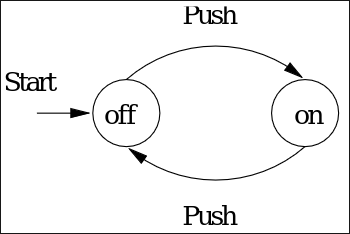
\includegraphics[width=.4\textwidth]{assets/intro-autom-stati-finiti.png}
    \caption{Automa a stati finiti per un interruttore on/off}\label{fig:intro-autom-stati-finiti}
\end{cimage}
% section Linguaggi di Programmazione (end)
%
\section{Linguaggi Naturali}\label{sec:i_linguaggi_naturali} % (fold)
\begin{definition}{Frasi Ambigue}{}
    Data una frase in input, anche se corretta, il suo albero sintattico può \textbf{non essere unico}
\end{definition}
\begin{definition}{Grammatiche Probabilistiche}{}
    Data una frase si può inferire l'\textbf{albero sintattico} più probabile
\end{definition}
%
\subsection{Language Model}\label{sub:i_language_model} % (fold)
Oltre a \textbf{grammatiche probabilistiche}, altri esempi classici di \ac{lm}:
\begin{itemize}
    \item \textbf{Bag of Words Model};
    \item \textbf{Hidden Markov Model} cioè automi a stati finiti probabilistici; 
\end{itemize}
Più recentemente \ac{lm} basati su \textbf{modelli neurali}:
\begin{itemize}
    \item nell'approccio classico basato su modelli probabilistici molta conoscenza linguistica viene \red{esplicitamente} rappresentata;
    \item nei modelli neurali le regolarità lessicali e sintattiche emergono \textbf{implicitamente} dei dati nell'apprendimento;
\end{itemize}
%
\subsubsection{Modelli Computazionali}\label{sub:i_modelli_computazionali} % (fold)
In un \ac{lm} è possibile fare \textbf{computazioni} tramite algoritmi:
\begin{itemize}
    \item \textbf{supervised/unsupervised learning};
    \item \textbf{inference/classification};
    \item \textbf{data generation} tramite campionamento distribuzioni;
\end{itemize}
In questo senso gli \ac{lm}, come tutti i \textbf{Generative Model}, sono \textbf{modelli computazionali}.
\emptyln{}
Ma anche i \textbf{Discriminative Model}, alternativi ai Generative Model, sono modelli computazionali.
% subsubsection Modelli Computazionali (end)
% subsection Language Model (end)
% section Linguaggi Naturali (end)
% chapter Intro (end)
